\section{Results and Discussion}
\label{results}

Through tens of thousands experiments across many signal-processing techniques (\textit{e.g.}~defences), random states, learning rates, model architectures, and attack configurations, we show that model defences generally fail to outperform the undefended model in either the benign or adversarial contexts, regardless of configuration; that the adversarial failure rate gains of larger ResNet configurations are driven by response time rather than true robustness; that these gains are dwarfed by the increase in training time; and that AFR models are a powerful tool for comparing model architectures and examining the effects of covariates.

\subsection{Attack and Defence Strength}
\begin{figure*}
    \centering
    \begin{subfigure}{0.49\textwidth}
        \centering
        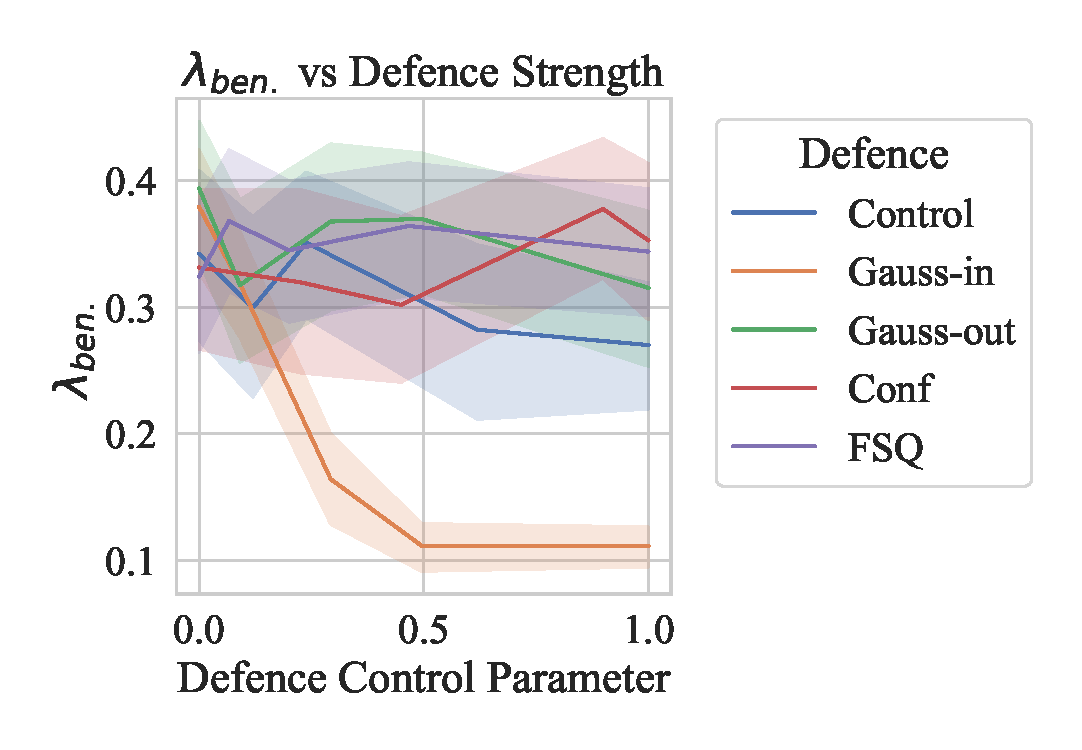
\includegraphics[width=\textwidth]{cifar/def_param_vs_accuracy.pdf}
    \end{subfigure}
    \begin{subfigure}{0.49\textwidth}
        \centering
        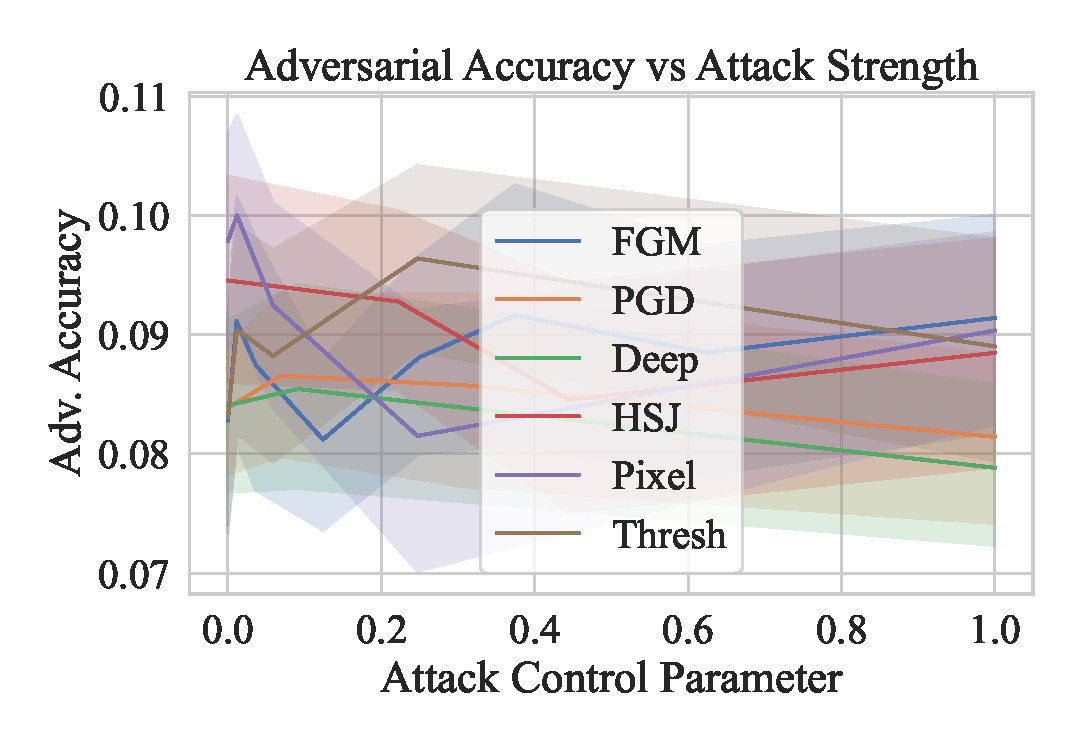
\includegraphics[width=\textwidth]{cifar/atk_param_vs_accuracy.pdf}
    \end{subfigure}
    \caption{This depicts the benign (unperturbed) and adversarial (perturbed) accuracies across all defences attacks, and models. The left shows how the benign accuracy varies with the defence strength where the control parameter describes the number of layers. The right shows the adversarial accuracy as a function of attack strength. The definition can be found in Eq.~\ref{eq:acc}}
    \label{fig:strength}
\end{figure*}


In Fig.~\ref{fig:strength}, we can see that no defence consistently outperforms the undefended (control) model (denoted in blue). Furthermore, the relationship between the defence control parameter and the benign accuracy is not monotonic, meaning that tuning is will be expensive. We can see that the relationship between the attack parameters and failure rate is not monotonic. However, all defences appear to perform much worse in the average adversarial case (middle~\&~right) than in the benign. Additionally we see that all attacks increase the failure rate to roughly 90\% or more (compared to the Control model in the benign case with less than 1\%). 

\subsection{Failure Rate}
\begin{figure*}
    \begin{subfigure}{0.50\textwidth}
        \centering
        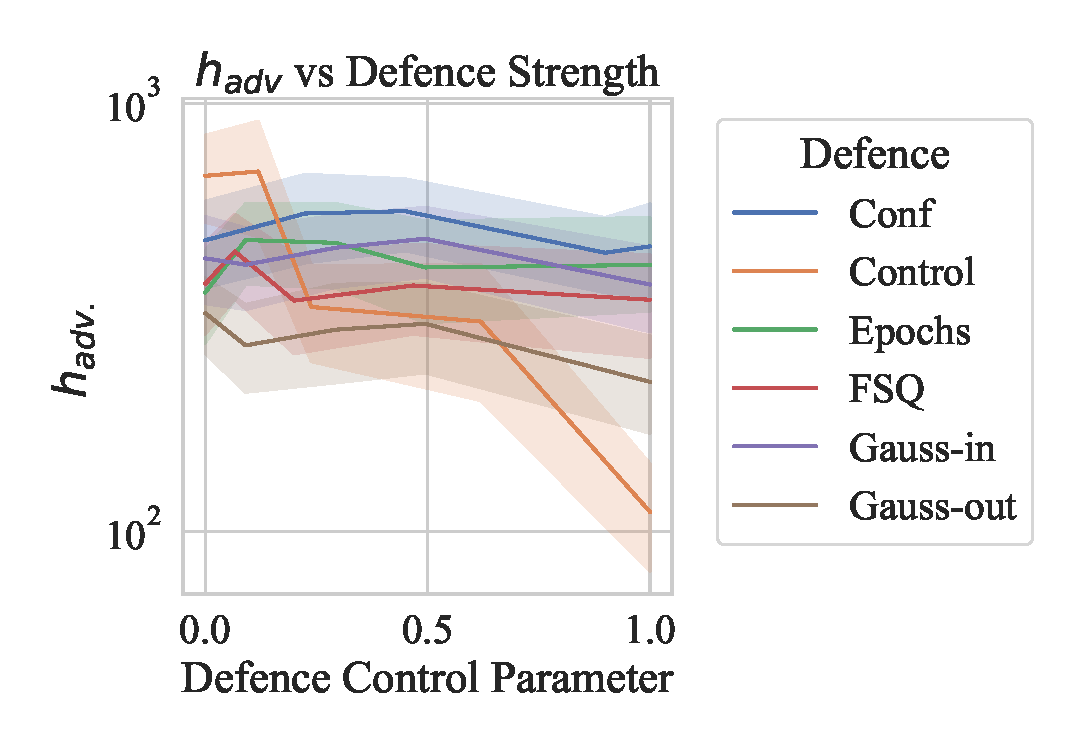
\includegraphics[width=\textwidth]{cifar/def_param_vs_adv_failure_rate.pdf}
    \end{subfigure}
    \begin{subfigure}{0.50\textwidth}
        \centering
        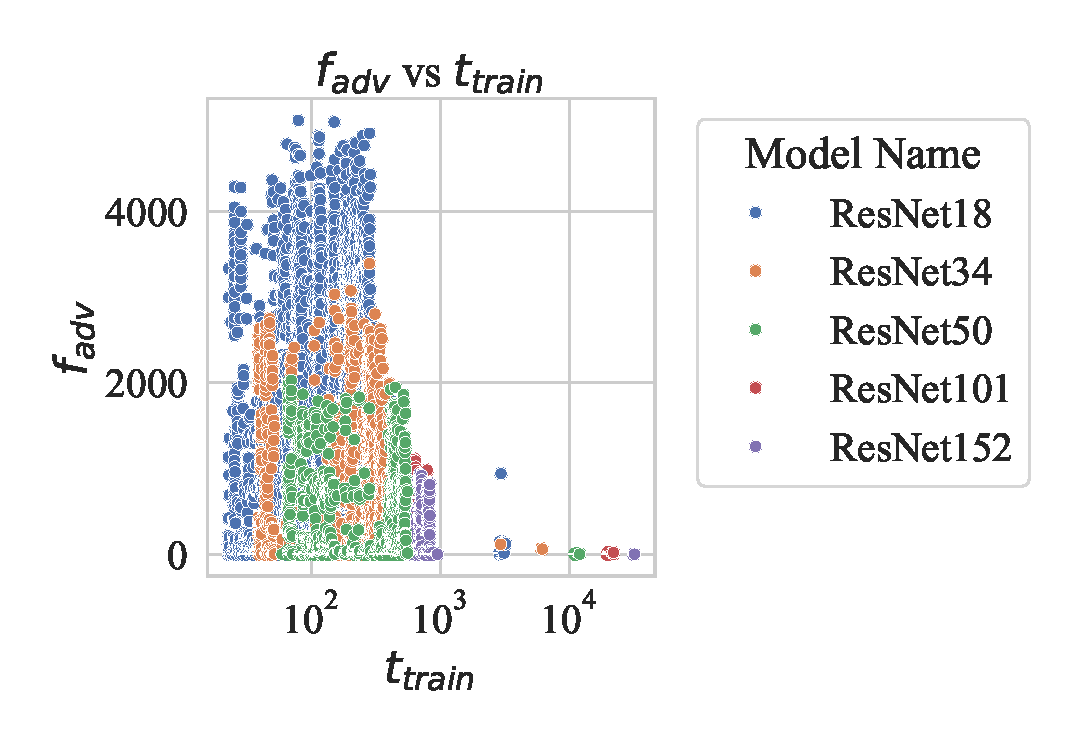
\includegraphics[width=\textwidth]{{cifar/adv_failure_rate_vs_train_time.pdf}}
    \end{subfigure}
    \caption{The left plot shows the adversarial failure rate (see: Eq.~\ref{eq:failure_rate}) as a function of the defence strength where the control parameter represents the number of model layers. The right plot depicts the adversarial failure rate as a function of training time and ResNet configuration.}
    \label{fig:failure_rate}
\end{figure*}
Fig.~\ref{fig:failure_rate} depicts all tested attacks, defences, and model configurations. Clearly, increasing the depth of the model architecture does little for adversarial robustness while universally increasing the training time. Furthermore, it reveals something surprising---that increasing the number of hidden layers tends to increase the failure rate--even across model architectures and all defences. Certain defences can outperform the control model- at the cost of expensive tuning- evidenced by the large variance in performance (see left side of Fig.~\ref{fig:failure_rate}). The right subplot of Fig.~\ref{fig:failure_rate} shows that there is no general relationship between training time and adversarial failure rate. We formalize this analysis  in the next subsection.


\begin{figure*}
    \centering
    \begin{subfigure}{.28\textwidth}
        \centering
        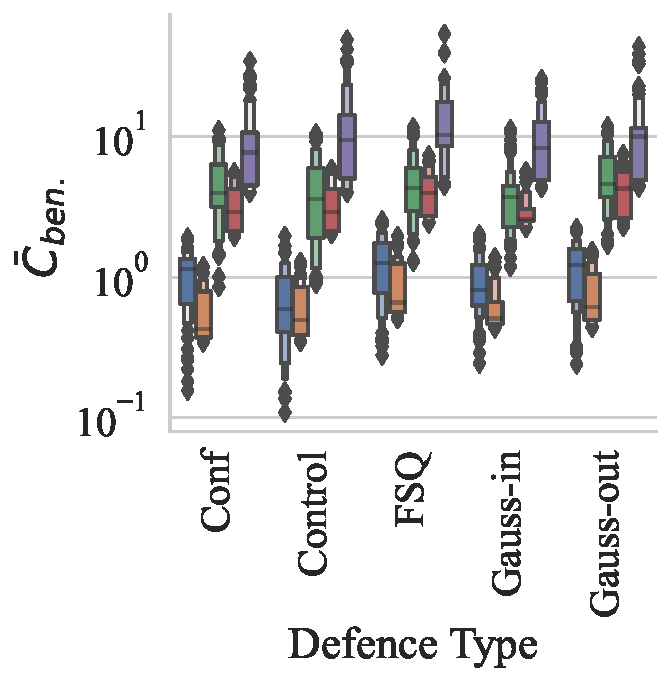
\includegraphics[width=\textwidth]{cifar/ben_failures_per_train_time_vs_defence_type.pdf}
    \end{subfigure}
    \begin{subfigure}{0.28\textwidth}
        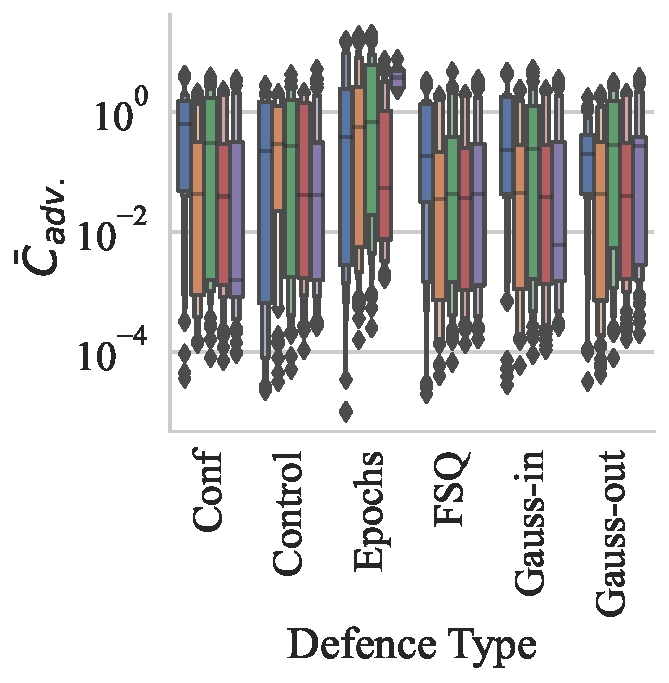
\includegraphics[width=\textwidth]{cifar/adv_failures_per_train_time_vs_defence_type.pdf}
        \centering
    \end{subfigure}
    \begin{subfigure}{0.42\textwidth}
        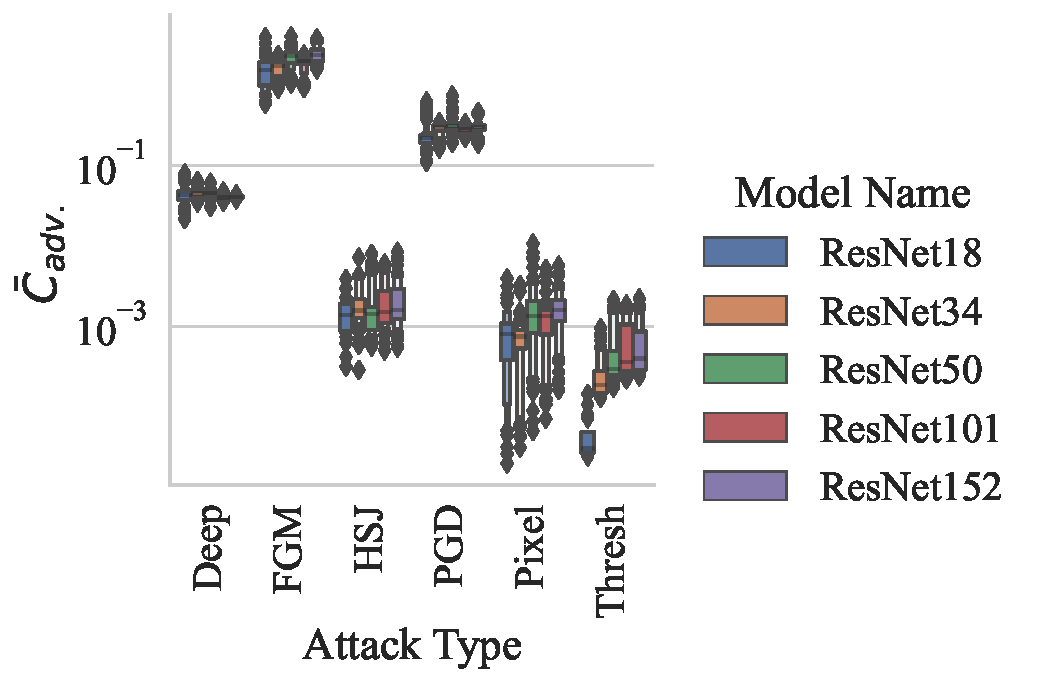
\includegraphics[width=\textwidth]{cifar/adv_failures_per_train_time_vs_attack_type.pdf}
        \centering
    \end{subfigure}
    \caption{This figure depicts the cost-normalized adversarial failure rate (see: Eq.~\ref{eq:cost}) across a variety of defences and attacks, where training time (middle~\&~right Figs.) and inference time (left figure) is a stand-in for cost (see Sec.~\ref{cost}).}
    \label{fig:failures_per_train_time}
\end{figure*}

Fig.~\ref{fig:failures_per_train_time} depicts the cost-normalized failure rate in both the benign (left) figure and adversarial cases (middle and right figure). Counter-intuitively, we see that the smallest model (ResNet18) tends to outperform both larger models (ResNet50 and ResNet152). Furthermore, we see that defence tuning is about as important as choosing the right type of defence, with all defences falling within the normal ranges of each other. However, adding noise to the model output (Gauss-out) tends to underperform relative to the control for all models. Likewise, the intersectional relationship between model choice and optimal defence is highlighted since the efficacy of a defence depends as much on model architecture as it does on hyperparameter tuning.  Furthermore, performance across all attacks is remarkably consistent with intra-class variation being smaller than inter-class variation almost universally across defences and model configurations. 

\subsection{AFR Models}
Fig.~\ref{fig:afr_models} reveals very similar estimates for the model parameters despite having different forms, suggesting that these parameter estimates reflect the true effect of these covariates on the failure rate. Table~\ref{tab:cifar} contains the performance of each of these models on the CIFAR10 dataset.  Sec.~\ref{appendix} contains the same data for MNIST. For both datasets, we can see that they are roughly comparable with regards to Concordance, but that Log-Normal model marginally outperforms the Weibull model when measured with AIC/BIC as well as the Concordance. 
In all cases, the expected mean is much larger than the median, indicating the long-tailed nature of these distributions. 
The concordance scores for all three distributions are in agreement as well, showing that these models outperform the assumption of time independence (e.g., Concordanace $> 0.5$). 
We then used the Log-Normal AFR to demonstrate the partial effect of the the number of layers on the survival time as in Fig.~\ref{fig:layers}. In that figure can clearly see that marginal hidden layers do increase the survival time. However, that seems to driven more by the resulting inference time (see Fig.~\ref{fig:afr_models}) than the number of model layers.
\begin{figure*}
    % \centering
    \begin{subfigure}{0.32\textwidth}
        \centering
        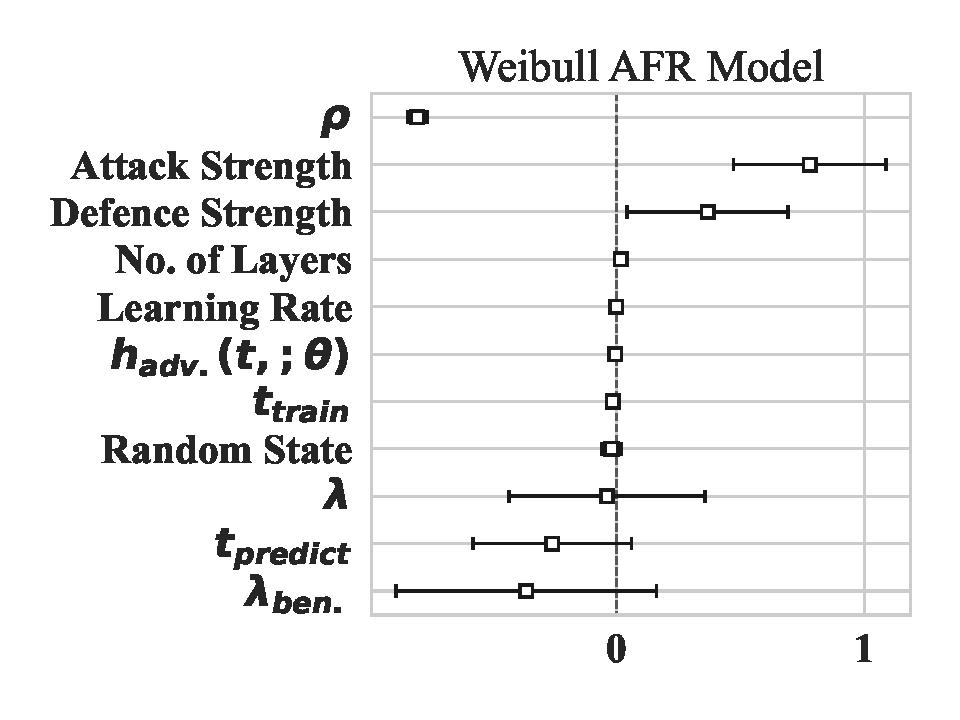
\includegraphics[width=\textwidth]{cifar/weibull_aft.pdf}
    \end{subfigure}%
    ~ 
    \begin{subfigure}{0.32\textwidth}
        \centering
        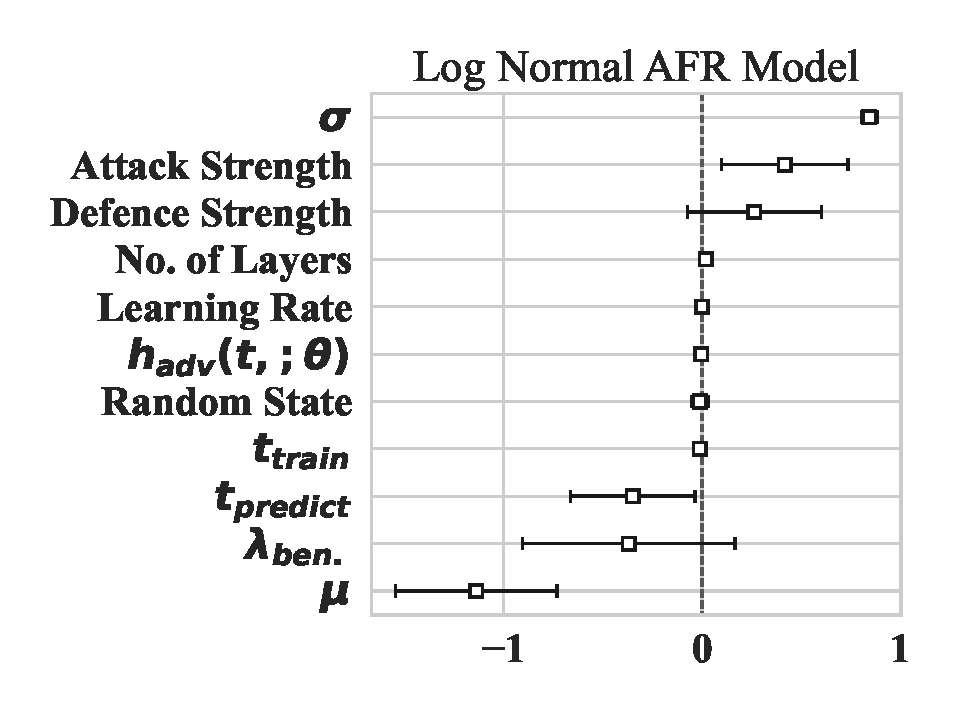
\includegraphics[width=\textwidth]{cifar/log_normal_aft.pdf}
    \end{subfigure}
    ~
    \begin{subfigure}{0.32\textwidth}
        \centering
        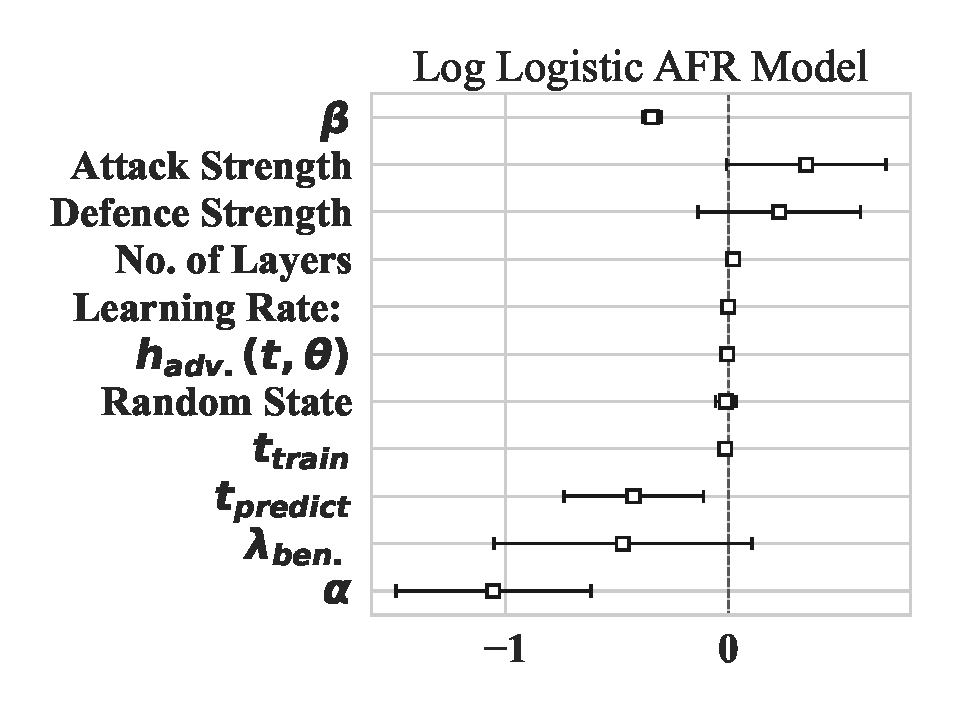
\includegraphics[width=\textwidth]{cifar/log_logistic_aft.pdf}
    \end{subfigure}
    
    \caption{The covariate estimates accelerated failure time models where the parameters $\rho$, $\lambda$, $\mu$, $\sigma$, $\alpha$, and $\beta$ represent the intercepts for those parameters as described in Sec.~\ref{afr_models} for the Weibull, Log-Normal, and Log-Logistic AFR Models. The coefficients represent the log scale effect of the covariates on the failure rate.}
    \label{fig:afr_models}
\end{figure*}

\begin{figure}
    % \begin{subfigure}
    %     \begin{table}
\caption{Comparison of AFR Models on the CIFAR dataset.}
\label{tab:cifar}
\begin{tabular}{l ccccc}
\toprule
 & AIC & Concordance & BIC & Mean $S(t;\theta)$ & Median $S(t;\theta)$ \\
\midrule
Weibull & 11359.69 & 0.79 & 11359.69 & 121.78 & 16.80 \\
LogNormal & 11137.47 & 0.80 & 11137.47 & 208.62 & 12.64 \\
LogLogistic & 11255.43 & 0.79 & 11255.43 & -- & 11.18 \\
\bottomrule
\end{tabular}
\end{table}

    % \end{subfigure}
    \centering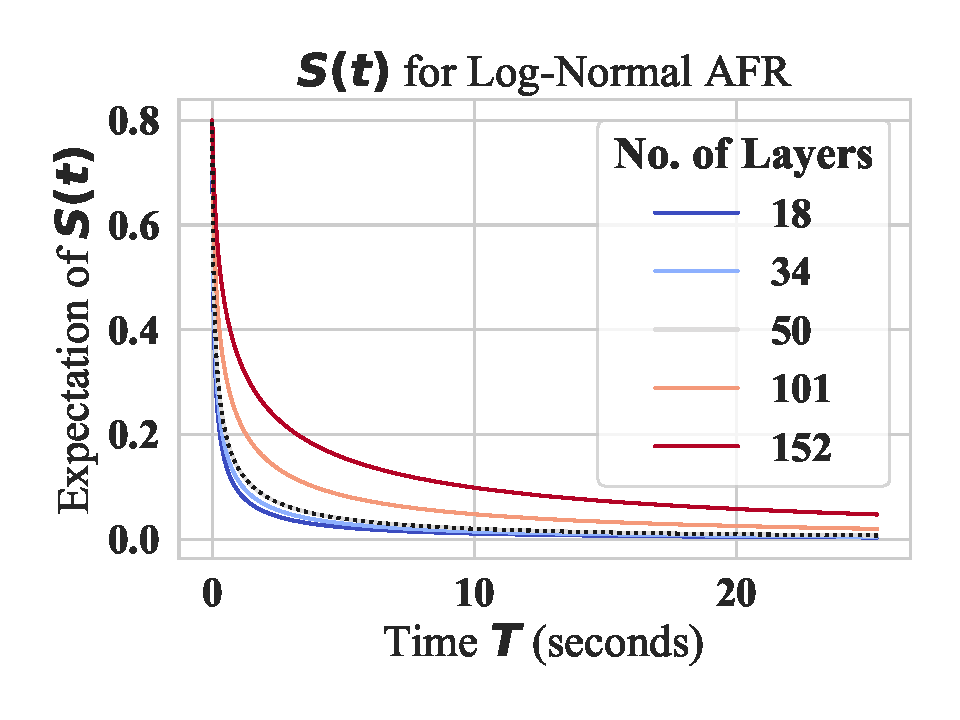
\includegraphics[width=.5\textwidth]{cifar/log_normal_partial_effects.pdf}
   \caption{This figure depicts the survival curve over time as a function of the number of model layers for the highest scoring model (the Log-Normal distribution). The partial effects plots of other models were excluded for space reasons, but the results were nearly identical.}
    \label{fig:layers}
\end{figure}
\begin{table}
\caption{Comparison of AFR Models on the CIFAR dataset.}
\label{tab:cifar}
\begin{tabular}{l ccccc}
\toprule
 & AIC & Concordance & BIC & Mean $S(t;\theta)$ & Median $S(t;\theta)$ \\
\midrule
Weibull & 11359.69 & 0.79 & 11359.69 & 121.78 & 16.80 \\
LogNormal & 11137.47 & 0.80 & 11137.47 & 208.62 & 12.64 \\
LogLogistic & 11255.43 & 0.79 & 11255.43 & -- & 11.18 \\
\bottomrule
\end{tabular}
\end{table}

% \begin{table}
\centering
\caption{Comparison of AFR Models on the MNIST dataset.}
\label{tab:mnist}
\begin{tabular}{lrrrrr}
\toprule
{} &      AIC &  Concordance &      BIC &  Mean \$S(t;\textbackslash theta)\$ &  Median \$S(t;\textbackslash theta)\$ \\
\midrule
Weibull      & 3.23e+03 &        0.929 & 3.23e+03 &                98.3 &                   1.1 \\
Log logistic & 2.98e+03 &        0.934 & 2.98e+03 &                71.4 &                  1.26 \\
Log normal   & 3.09e+03 &        0.934 & 3.09e+03 &                77.6 &                  1.27 \\
\bottomrule
\end{tabular}
\end{table}



